The frequency sweeps and the models of \nameref{sec:four} point in the same direction: phase-locking tends to affect the internal representation but does not appear to propagate to the forecast output.

On the behavioural side, locked frequencies are not systematically attenuated in the rollout. In several geometries the model reconstructs them as well as their unlocked neighbours, contrary to what the degeneracy alone would predict. The representational side points toward a different pattern: the prequential codelength at a locked frequency tends to be higher than at an unlocked one, suggesting that the internal state carries a measurable cost at those sites. This split, representation penalised and forecast intact, is the pattern the evidence points to, and the per-generator and per-geometry evidence follows.

The phase of the input signal does not appear to modulate the deficit appreciably, consistent with $H2$: the posterior for $\sigma_\phi$ in \autoref{fig:phasePosterior} lies inside the region of practical equivalence (ROPE). It concentrates well below the threshold and is far tighter than the prior it started from, so the data and not the prior place it there, and the eight per-phase offsets $u_p$ are not separable from one another. The size of the deficit therefore follows from the geometry and from the frequency, and not from where in its cycle the signal begins, which is what licences the remaining models to average over phase and which also removes phase randomisation from the mitigations available to an operator.

The token-collapse dips align with the stride grid and shift when the stride changes, consistent with $H3a$, and \autoref{fig:combs} shows the pattern holding across configurations and generators; the scaling law of the patch branch is not identified in the runs fitted for this deliverable.

\begin{figure*}[!b]
    \centering
    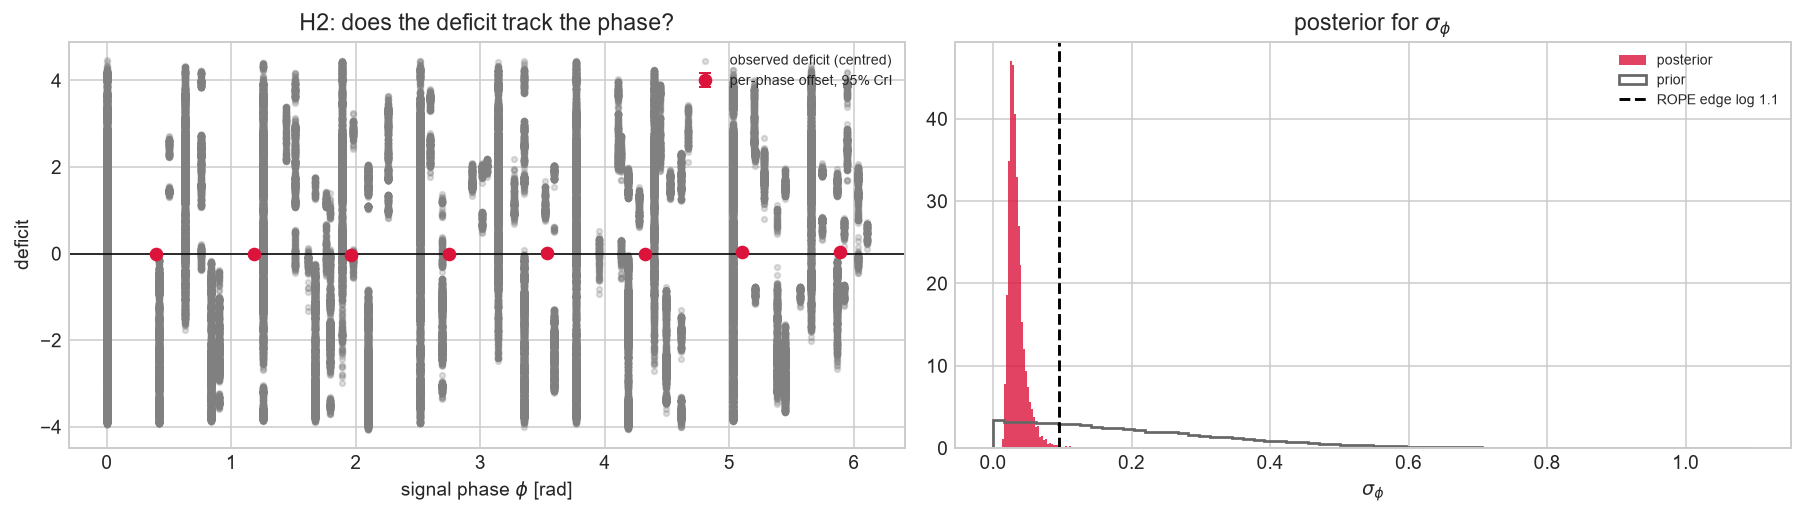
\includegraphics[width=0.92\textwidth]{figures/FIG_H2_phase.png}
    \caption{Posterior for the phase term of $H2$. On the left the observed deficit against the signal phase $\phi$, with the per-phase offset $u_p$ and its $95\%$ credible interval; on the right the posterior for $\sigma_\phi$ against its prior, the dashed line marking the ROPE edge at $\log 1.1$. Both panels pool every configuration fitted, so the estimate is not conditioned on a single geometry. Model~C has not met the convergence thresholds of \nameref{sec:four}, so the posterior is shown as provisional.}
    \label{fig:phasePosterior}
\end{figure*}

\begin{figure*}[p]
    \centering
    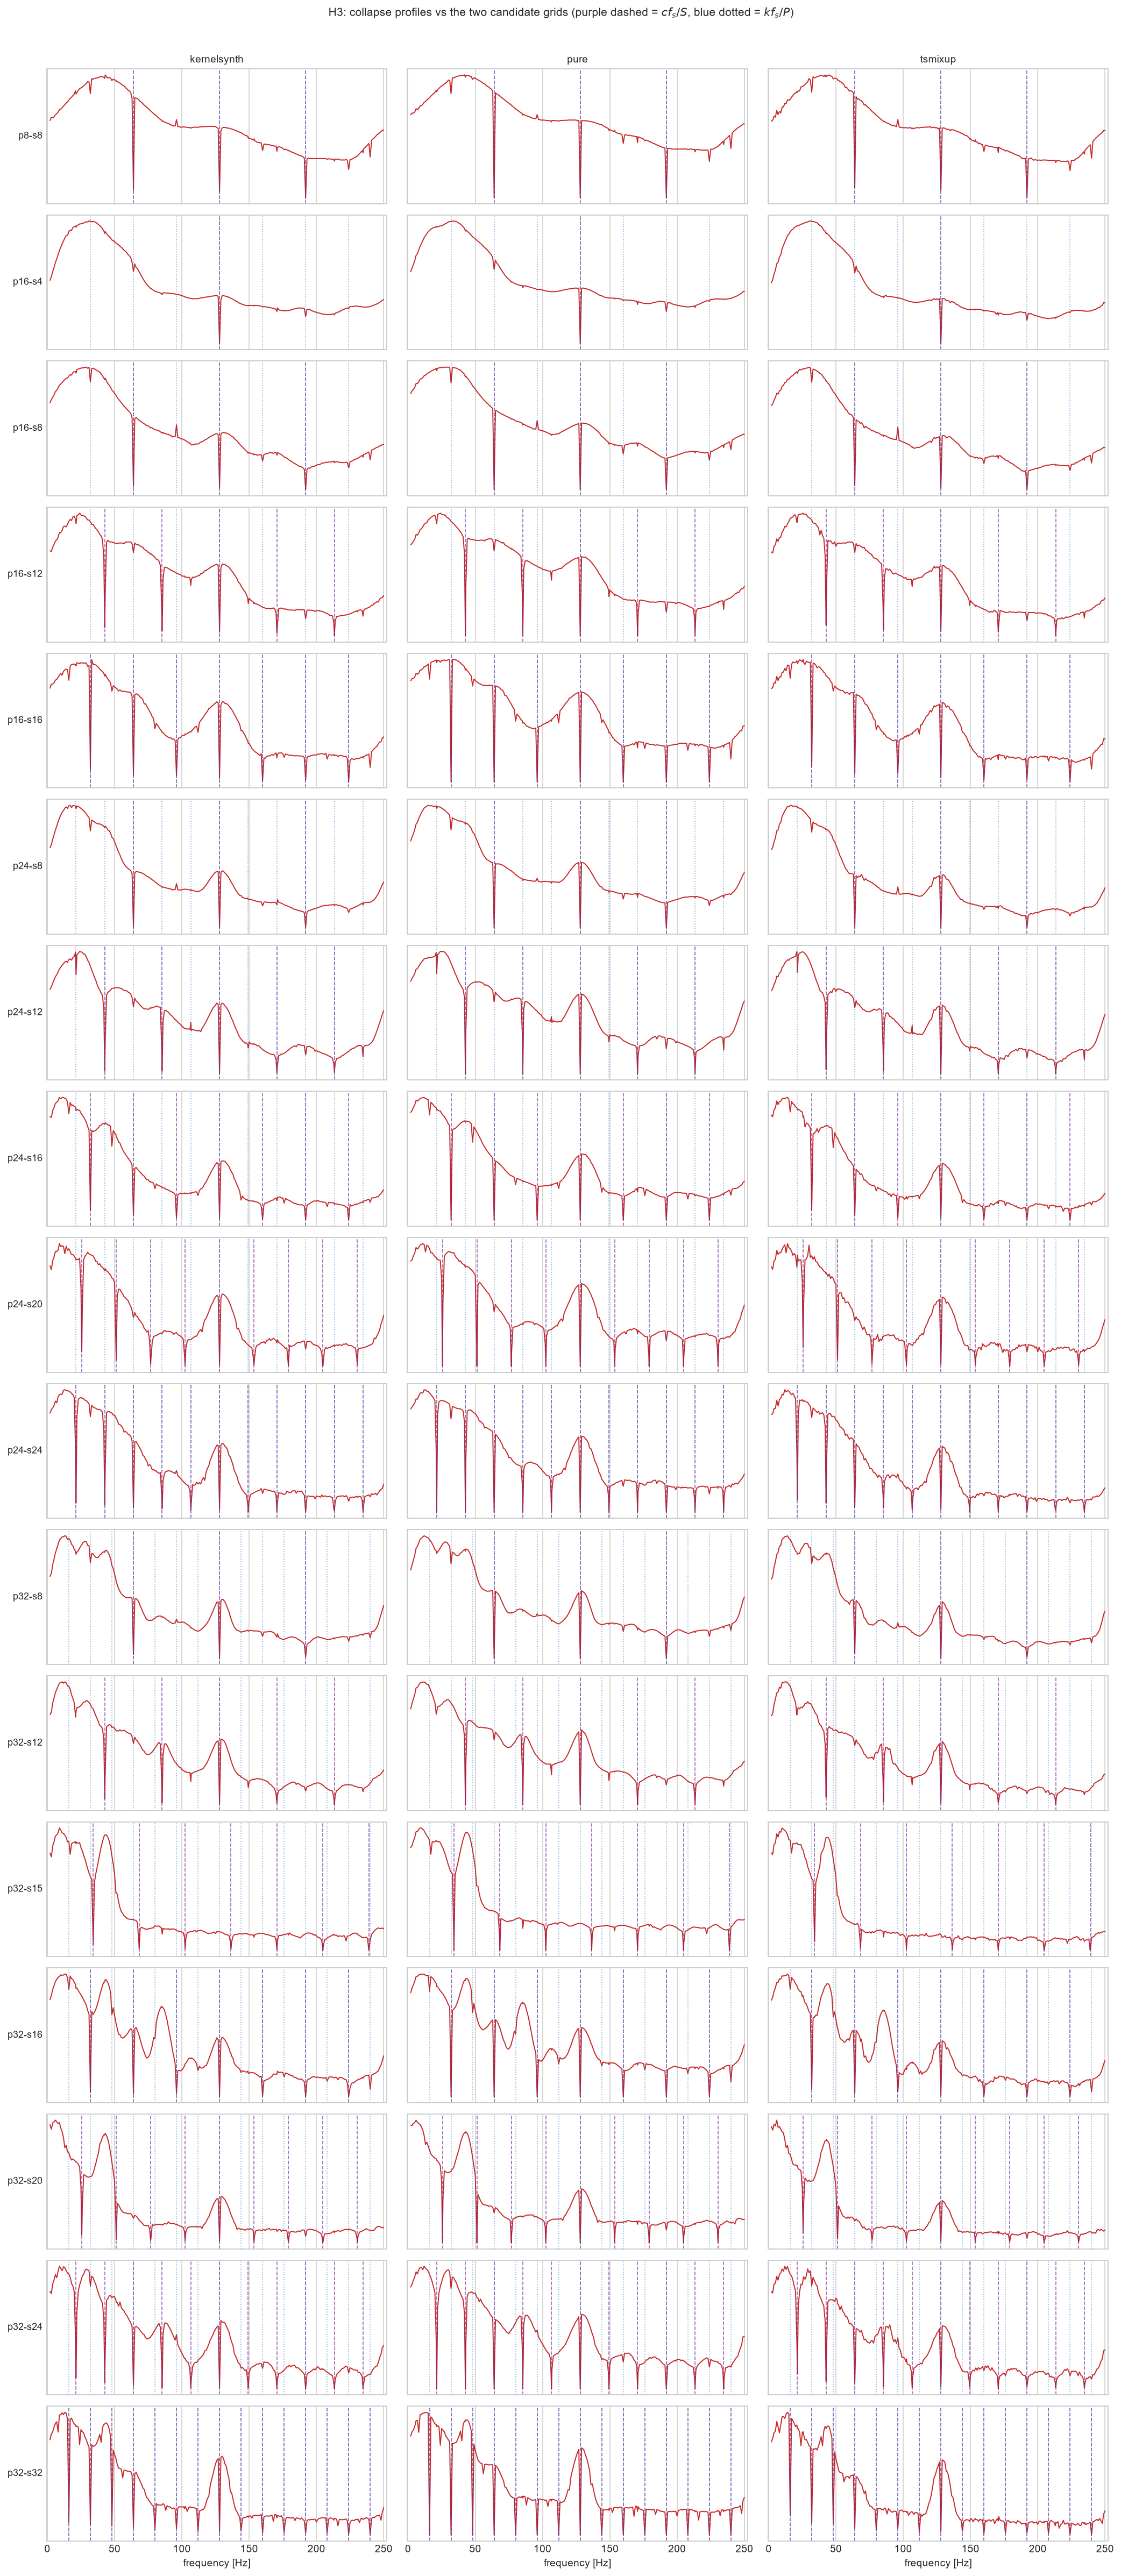
\includegraphics[height=0.88\textheight]{figures/FIG_H3_combs.png}
    \caption{Collapse profiles against the two candidate grids. Rows are the fitted configurations and columns the three generators; each panel plots the profile over the sweep band, with the stride grid $cf_s/S$ dashed and the patch grid $kf_s/P$ dotted. A dip that sits on the dashed grid and follows it as the stride changes belongs to the stride branch. The run shown is provisional: it does not cover every configuration of \autoref{tab:hfModels} and it includes runs the final analysis excludes.}
    \label{fig:combs}
\end{figure*}

Models~A and~C have not reached the preregistered convergence thresholds; their estimands are nonetheless consistent with the converged representational model~(B) and with the independent frequentist sweeps, so the qualitative conclusions hold provisionally. Consolidated posteriors or, if convergence remains out of reach, a documented limitation and fall-back on the frequentist evidence will follow.
